\chapter{Deep Declarative Network}
\label{cha:ddn}
In this chapter, we will cover the structure and nodes in the deep declarative network: from its learning process to the back-propagation.
\par Before delving into the details of the back-propagation in different constraints cases, we give an overview of the deep declarative network in Section~\ref{sec:overview-ddn}. In particular, the basic structure of the network and the details of declarative nodes are described according to \cite{SG:19}. The learning progress of the network is also given. We hope this will give readers a better sense of what is the deep declarative network and how it works. 
\par In Section~\ref{sec:bp}, we present the details of the back-propagation in different constrained problems. The gradient computation results are based on the implicit differentiation and different in constrained problems. We discuss this part based on the regular solution and compare it with the general solution in the previous chapter. 
\par Next we present the examples of constrained optimization problems with both linear and non-linear, equality and inequality constraints in Section~\ref{sec:example}. We also provide more implementation details of the deep declarative nodes. 
\par Finally, we summarize the deep declarative network and its solution in different constrained problems under the regular point. 


\section{An Overview of Deep Declarative Network}
\label{sec:overview-ddn}
\subsection{Declarative Node}
In deep declarative network, it defines the solution of a constrained optimization problem with parameter $x \in \mathbb{R}^n$ as the output of each node $y \in \mathbb{R}^m$. The general optimization problem can be defined as 
\begin{equation}
    y \in \underset{u \in C}{\arg \min } f(x, u)
\end{equation}
where $f$ is the objective function $f: \mathbb{R}^n \times \mathbb{R}^m \rightarrow \mathbb{R}$, and $C \in \mathbb{R}^m$ is the set of constraints parameterized by $x$. 
\par Apart from the traditional forward processing mapping node, deep declarative node does not explicitly define the transforming function from the input to the output. It defines the input-output relationship implicitly by an objective and constriants optimization problem, where the solution of the problem is the output. 
\begin{figure}
    \label{fig:ddn}
    \centering
    \tikzset{every picture/.style={line width=0.75pt}} %set default line width to 0.75pt        

    \begin{tikzpicture}[x=0.75pt,y=0.75pt,yscale=-1,xscale=1]
    %uncomment if require: \path (0,300); %set diagram left start at 0, and has height of 300

    %Rounded Rect [id:dp5847695584847934] 
    \draw   (233,118.5) .. controls (233,113.81) and (236.81,110) .. (241.5,110) -- (421,110) .. controls (425.69,110) and (429.5,113.81) .. (429.5,118.5) -- (429.5,177.14) .. controls (429.5,181.84) and (425.69,185.64) .. (421,185.64) -- (241.5,185.64) .. controls (236.81,185.64) and (233,181.84) .. (233,177.14) -- cycle ;
    %Straight Lines [id:da8797940676718146] 
    \draw    (197.5,135.64) -- (230.5,135.64) ;
    \draw [shift={(232.5,135.64)}, rotate = 180] [color={rgb, 255:red, 0; green, 0; blue, 0 }  ][line width=0.75]    (10.93,-3.29) .. controls (6.95,-1.4) and (3.31,-0.3) .. (0,0) .. controls (3.31,0.3) and (6.95,1.4) .. (10.93,3.29)   ;
    %Straight Lines [id:da5288114309680509] 
    \draw    (232.5,165.64) -- (200.5,165.64) ;
    \draw [shift={(198.5,165.64)}, rotate = 360] [color={rgb, 255:red, 0; green, 0; blue, 0 }  ][line width=0.75]    (10.93,-3.29) .. controls (6.95,-1.4) and (3.31,-0.3) .. (0,0) .. controls (3.31,0.3) and (6.95,1.4) .. (10.93,3.29)   ;
    %Straight Lines [id:da8485926924080154] 
    \draw    (429.5,135.64) -- (462.5,135.64) ;
    \draw [shift={(464.5,135.64)}, rotate = 180] [color={rgb, 255:red, 0; green, 0; blue, 0 }  ][line width=0.75]    (10.93,-3.29) .. controls (6.95,-1.4) and (3.31,-0.3) .. (0,0) .. controls (3.31,0.3) and (6.95,1.4) .. (10.93,3.29)   ;
    %Straight Lines [id:da8644978866807145] 
    \draw    (463.5,165.64) -- (431.5,165.64) ;
    \draw [shift={(429.5,165.64)}, rotate = 360] [color={rgb, 255:red, 0; green, 0; blue, 0 }  ][line width=0.75]    (10.93,-3.29) .. controls (6.95,-1.4) and (3.31,-0.3) .. (0,0) .. controls (3.31,0.3) and (6.95,1.4) .. (10.93,3.29)   ;
    %Straight Lines [id:da03877231252818136] 
    \draw    (300,78.5) -- (300,107.64) ;
    \draw [shift={(300,109.64)}, rotate = 270] [color={rgb, 255:red, 0; green, 0; blue, 0 }  ][line width=0.75]    (10.93,-3.29) .. controls (6.95,-1.4) and (3.31,-0.3) .. (0,0) .. controls (3.31,0.3) and (6.95,1.4) .. (10.93,3.29)   ;
    %Straight Lines [id:da34598442566525556] 
    \draw    (350,109.64) -- (350,80.64) ;
    \draw [shift={(350,78.64)}, rotate = 450] [color={rgb, 255:red, 0; green, 0; blue, 0 }  ][line width=0.75]    (10.93,-3.29) .. controls (6.95,-1.4) and (3.31,-0.3) .. (0,0) .. controls (3.31,0.3) and (6.95,1.4) .. (10.93,3.29)   ;

    % Text Node
    \draw (260,140) node [anchor=north west][inner sep=0.75pt]   [align=left] {$\displaystyle y\ \in \underset{u\ \in \ C}{\arg\min} f( x,\ u;\ \theta ) \ $};
    % Text Node
    \draw (175,130) node [anchor=north west][inner sep=0.75pt]   [align=left] {$\displaystyle x$};
    % Text Node
    \draw (145,158) node [anchor=north west][inner sep=0.75pt]   [align=left] {$\displaystyle \operatorname{D} J( x)$};
    % Text Node
    \draw (475,130) node [anchor=north west][inner sep=0.75pt]   [align=left] {$\displaystyle y$};
    % Text Node
    \draw (472,158) node [anchor=north west][inner sep=0.75pt]   [align=left] {$\displaystyle \operatorname{D} J( y)$};
    % Text Node
    \draw (295,58) node [anchor=north west][inner sep=0.75pt]   [align=left] {$\displaystyle \theta $};
    % Text Node
    \draw (332,55) node [anchor=north west][inner sep=0.75pt]   [align=left] {$\displaystyle \operatorname{D} J( \theta )$};
    \end{tikzpicture}

    \caption{End-to-end learnable declarative node}
\end{figure}
\par Figure~\ref{fig:ddn} shows the forward and backward pass of the declarative node. In the forward evaluation pass, the output of the declarative $y$ is computed as the solution of some minimization problem $f(x, u; \theta)$. We use $\operatorname{D}$ to denote the total derivative with respect to the independent variables. Therefore, in the backward pass, the gradient of the global objective function with respect to the output $\operatorname{D}J(y)$ is back-propagated. Its value is computed through the chain rule based on the gradients with respect to the input $\operatorname{D}J(x)$ and parameters $\operatorname{D}J(\theta)$.
\par Since the definition of deep declarative nodes is very general, it can be embedded within another network for solving subproblems such as robust fitting. However, we may not be able to find the gradient when the feasible set is discrete, or the declarative node is low efficiency to evaluate. As non-regular solution cases, the nonexistent gradient problem will be discussed in the next part. In the next subsection, the learning details of the deep declarative network are described. 

\subsection{Learning}



\section{Back-propagation Through Declarative Nodes}
\label{sec:bp}

\subsection{Unconstrained}
\subsection{Equality Constrained}
\subsection{Inequatlity Constrained}

\section{Examples of Declarative Nodes}
\label{sec:example}

\subsection{Implementation Details}
\subsection{Equality Constrained}

\subsection{Inequatlity Constrained}

\section{Summary}
